\documentclass[12pt]{beamer}

\usepackage{xcolor}
\usepackage{layouts}
\usepackage{minted}
\usepackage[most]{tcolorbox}
\usepackage{natbib}
\tcbuselibrary{minted}
\usemintedstyle{xcode}
\setminted{
    fontfamily=helvetica
}


\usepackage{booktabs}

\usepackage{outlines}
\usepackage{hyperref}
\usepackage{graphicx}
\usepackage{amsmath}
\usepackage{makecell}

% justify
\usepackage{ragged2e}
\justifying\let\raggedright\justifying


% outline space
\makeatletter
\renewenvironment{outline}[1][]{%
  \ifthenelse{\equal{#1}{}}{}{\renewcommand{\ol@type}{#1}}%
  \ol@z%
  \newcommand{\0}{\ol@toz\ol@z}%
  \newcommand{\1}{\vspace{\dimexpr\outlinespacingscalar\baselineskip-\baselineskip}\ol@toi\ol@i\item}%
  \newcommand{\2}{\ol@toii\ol@ii\item}%
  \newcommand{\3}{\ol@toiii\ol@iii\item}%
  \newcommand{\4}{\ol@toiiii\ol@iiii\item}%
}{%
  \ol@toz\ol@exit%
}
\makeatother




\renewcommand\theadalign{bc}
\renewcommand\theadfont{\bfseries}
\renewcommand\theadgape{\Gape[4pt]}
\renewcommand\cellgape{\Gape[4pt]}

\beamertemplatenavigationsymbolsempty

\newif\ifsectiontitlepage
\sectiontitlepagetrue

\newcommand{\nosectiontitlepage}{\sectiontitlepagefalse}


\AtBeginSection[]{
\ifsectiontitlepage
  \begin{frame}
  \tableofcontents[currentsection, hideothersubsections]
  \end{frame}
\fi
}



%%

% color
\definecolor{coreFontMain}{RGB}{26,26,26}
\definecolor{coreFontSub}{RGB}{106,106,106}
\definecolor{coreBackgroundLight}{RGB}{230,230,230}
\definecolor{coreBackground}{RGB}{255,255,255}

% heading
\newlength{\headerheight}
\setlength{\headerheight}{0.094\paperheight}


\setbeamerfont{frametitle}{size=\fontsize{12}{14.4}}
\setbeamertemplate{frametitle}
{%
\nointerlineskip
\begin{beamercolorbox}[wd=\paperwidth,left,sep=0pt]{}
\begin{tcolorbox}[enhanced,frame hidden, 
    borderline south={0.5pt}{0pt}{coreFontSub},
    colback=coreBackground, coltext=coreFontSub,height=\headerheight,notitle,left*=0.05\paperwidth,boxsep=0pt,bottom=0pt,halign=left,valign=bottom,before skip=0pt,after skip=0pt, before upper=\strut]
    \usebeamercolor{frametitle}\insertframetitle
\end{tcolorbox}
\end{beamercolorbox}
}


% footer
\newlength{\footerheight}
\setlength{\footerheight}{0.06\paperheight}
\setbeamercolor{footer}{bg=coreBackgroundLight, fg=coreFontMain}

\setbeamerfont{footline}{size=\fontsize{10}{12}}
\setbeamertemplate{footline}
{%
\begin{beamercolorbox}[sep=0pt,wd=\paperwidth,center]{footer}
%\begin{minipage}[c][\footerheight]{\textwidth}

\begin{minipage}[c][\footerheight]{\textwidth}
    \fontsize{8}{9.6}\selectfont
    \centering
    \insertframenumber/\inserttotalframenumber            
\end{minipage}
    
%\end{minipage}
\end{beamercolorbox}
}



% Title Page

% header
% \newlength{\titleheaderheight}
% \setlength{\titleheaderheight}{0.0666667\paperheight}
% \setbeamercolor{header}{bg=coreBackgroundLight}

%% logo
\newlength{\logoheight}
\setlength{\logoheight}{0.297\paperheight}

%% title
\setbeamercolor{title}{fg=coreFontMain}
\setbeamerfont{title}{size=\fontsize{18.14}{21.768}}
\newlength{\titleheight}
\setlength{\titleheight}{0.19\paperheight}


%% meta
\newlength{\metaheight}
\setlength{\metaheight}{0.21\paperheight}
\setbeamercolor{meta}{fg=coreFontSub}
\setbeamerfont{meta}{size=\fontsize{9.07}{10.884}}

%% contact
\newlength{\contactheight}
\setlength{\contactheight}{0.193333\paperheight}



\makeatletter
% \newcommand{\iftitlegraphicisempty}{%
%   \ifx\@empty\inserttitlegraphic%
%     \expandafter\@firstoftwo%
%   \else%
%     \expandafter\@secondoftwo%
%   \fi%
% }
\setbeamertemplate{title page}{
% \nointerlineskip
% 
\ifx\@empty\inserttitlegraphic%
    \setlength{\titleheight}{0.4\paperheight}
    \setlength{\metaheight}{0.4\paperheight}%
    \setbeamerfont{meta}{size=\fontsize{11}{13.2}}
\else%
    \inserttitlegraphic%
\fi%

\begin{tcolorbox}[enhanced,frame hidden, borderline south={0.5pt}{0pt}{coreFontMain}, colback=coreBackground,height=\titleheight,boxsep=0pt,notitle,halign=flush center,valign=center, bottom=-30pt,before skip=0pt,after skip=0pt, coltext=coreFontMain]
\usebeamercolor{title}
\usebeamerfont{title}\inserttitle
\end{tcolorbox}

\usebeamercolor[fg]{meta}{
\begin{minipage}[c][\metaheight]{\textwidth}
    \usebeamerfont{meta}
    \centering
    \insertauthor \linebreak
    \insertinstitute \linebreak
    \insertdate
\end{minipage}
}


\begin{tcolorbox}[enhanced,frame hidden, colback=coreBackground,height=\contactheight,notitle,halign=flush center,valign=top,before skip=0pt,after skip=0pt,top=-5pt]
\begin{tabular}{ccc}
\href{mailto:zhangbohan@buaa.edu.cn}{
\includegraphics[height=3mm]{bohanbeamerstyle/figures/mail.png}} & \href{https://github.com/angelpone}{
\includegraphics[height=3mm]{bohanbeamerstyle/figures/github.png}} & \href{https://twitter.com/zhangbhangel}{
\includegraphics[height=3mm]{bohanbeamerstyle/figures/Twitter.png}}
\end{tabular}

\end{tcolorbox}


% \begin{beamercolorbox}[sep=2pt,center,wd=\paperwidth,ht=\footerheight]{footer}
% \tiny
% \insertframenumber/\inserttotalframenumber
% \end{beamercolorbox}
% \nointerlineskip
}


% 
\setbeamercolor{normal text}{bg=coreBackground,fg=coreFontMain}

% itemize
\setbeamertemplate{itemize items}[circle]

\setlength{\leftmarginii}{10pt}
\setbeamercolor{itemize item}{fg=coreFontMain}
\setbeamercolor{itemize subitem}{fg=coreFontMain}
\setbeamercolor{itemize subsubitem}{fg=coreFontMain}



\usepackage{blkarray}
% \titlegraphic{ss}
\title{Discrete Forecast Reconciliation}
\author{Bohan Zhang}
\institute{Beihang University \\ 
IIF Workshop on Forecast Reconciliation}
\date{September 7, 2023}

% style setting
\nosectiontitlepage
\def\outlinespacingscalar{1.3}
\setbeamertemplate{blocks}[rounded][shadow=false]
\setbeamercolor{block title}{bg=teal, fg=white}
\setbeamercolor{block body}{bg=teal!10}
\setbeamerfont{block title}{size=\fontsize{10}{12}}
\setlength{\leftmargini}{10pt}

\begin{document}

\begin{frame}[plain]

    \maketitle

\end{frame}



\begin{frame}
    \frametitle{Collaborate with}
    \fontsize{9}{10.8}\selectfont
    \begin{table}
    \begin{tabular}{ccc}
        
\includegraphics[width=0.3\textwidth]{figures/tas.jpg} &
        
\includegraphics[width=0.3\textwidth]{figures/yfkang.png} &
        
\includegraphics[width=0.3\textwidth]{figures/fengli.png} \\
        \begin{minipage}[t]{0.3\textwidth}\centering Anastasios Panagiotelis \\ University of Sydney \end{minipage} &
        \begin{minipage}[t]{0.3\textwidth}\centering Yanfei Kang \\ Beihang University \end{minipage} &
        \begin{minipage}[t]{0.3\textwidth}\centering Feng Li \\ Central University of \\ Finance and Economics \end{minipage}
    \end{tabular}
    \end{table}

\end{frame}


\begin{frame}
    \frametitle{CONTENTS}
    \tableofcontents
\end{frame}


\section{Introduction}
\begin{frame}
\frametitle{Motivation}
\framesubtitle{the problem}

\begin{outline}
\1 Non-negative and discrete-valued time series, particularly those with low counts, commonly arise in various fields. Examples include:
\2 occurrences of “black swan” events
\2 intermittent demand in the retail industry

\1 Despite the great concern of hierarchical forecasting in these applications, limited research have been conducted.


\end{outline}

\end{frame}

\begin{frame}
\frametitle{Motivation: the lesson learned from reconciliation approach}


\begin{outline}
    \0 The forecast reconciliation approach
    \1 first produces base forecasts for each series in the hierarchy; then optimally reconciles the base forecasts through projection;
    \1 utilises forecast combination, which improves forecast accuracy and reduces the risk of model misspecification;
    \1 has been shown to improve forecast accuracy in various applications.
    \0 But it was designed for continuous-valued HTS and can not be directly applied to discrete-valued HTS: \textit{projection} may produce non-integer and negative forecasts.
\end{outline}

\end{frame}


\begin{frame}
\frametitle{Motivation: probabilistic forecasting}
    \begin{outline}

        \1 While point and interval forecasts are most widely applied in practice, attention has been shifted towards full predictive distribution.
        \1 When forecasting discrete-valued time series, it is also more natural to produce predictive distribution.

    \end{outline}

\end{frame}


\begin{frame}{Related Work}

A series of work on forecast reconciliation for count HTSs:

\begin{itemize}
    \fontsize{9}{10.2}\selectfont
    \item Corani, G., Azzimonti, D., Rubattu, N., \& Antonucci, A. (2022). Probabilistic Reconciliation of Count Time Series (arXiv:2207.09322). arXiv.
    \item Zambon, L., Azzimonti, D., \& Corani, G. (2022). Efficient probabilistic reconciliation of forecasts for real-valued and count time series (arXiv:2210.02286). arXiv.
    \item Zambon, L., Agosto, A., Giudici, P., \& Corani, G. (2023). Properties of the reconciled distributions for Gaussian and count forecasts (arXiv:2303.15135). arXiv.
\end{itemize}

The proposed framework conditions base probabilistic forecasts of the most disaggregated series on base forecasts of aggregated series. However, it fails to restore the dependence structure within hierarchical time series.

\end{frame}

\begin{frame}{Contribution}

To address these concerns, we 

\begin{itemize}
    \item introduce the definition of \textit{coherent domain and coherent forecasts} in the context of multivariate discrete random variables.
    \item propose a discrete forecast reconciliation framework.
    \item develop the DFR and Stepwise DFR (SDFR) algorithms to train the reconciliation matrix.
    \item extend the top-down and bottom-up method to discrete probabilistic setting for comparison.
    \item verify the applicability of the algorithms in simulation experiments and real-world applications.
\end{itemize}

\end{frame}



\section{Coherent discrete predictive distribution}

\begin{frame}{Coherent and incoherent domain for discrete HTS}
\begin{table}
    \fontsize{10}{12}\selectfont
\begin{tabular}{ll}
    \toprule
    HTS & $\mathbf{Y}=(Y_1,Y_2,\dots,Y_n)'$ \\
    basis (e.g., bottom-level) time series & $\mathbf{Y}_b = (Y_1,Y_2,\dots,Y_{m})'$ \\
    domain of $i$-th variable & $\mathcal{D}(Y_i) = \{0,1,\dots,D_i\}$ \\\bottomrule
\end{tabular}
\end{table}


    Complete domain of $\mathbf{Y}$ is the Cartesian product of domains of all variables.
    \[
        \hat{\mathcal{D}}(\mathbf{Y}) = \{0,\dots,D_1\}\times \dots\times \{0,\dots,D_n\} \quad q:= |\hat{\mathcal{D}}(\mathbf{Y})|
    \]

    Coherent domain of $\mathbf{Y}$ is a subset of $\hat{\mathcal{D}}(\mathbf{Y})$, in which every point respects the aggregation constraints.
    \[
        \tilde{\mathcal{D}}(\mathbf{Y}) = \{\mathbf{y} | \mathbf{y}\in \hat{\mathcal{D}}(\mathbf{Y}), S\mathbf{y}_b = \mathbf{y}\} \quad r:=|\tilde{\mathcal{D}}(\mathbf{Y})|
    \]

    Incoherent domain of $\mathbf{Y}$
    \[
        \bar{\mathcal{D}}(\mathbf{Y}) = \hat{\mathcal{D}}(\mathbf{Y}) \backslash \tilde{\mathcal{D}}(\mathbf{Y})
    \]


\end{frame}


\begin{frame}{Example}
\begin{block}{Variables}
\[
\begin{aligned}
  \mathcal{D}(Y_1) = \{0, 1\}, \mathcal{D}(Y_2) = \{0, 1\}, \\
  Y_3=Y_1+Y_2, \mathcal{D}(Y_3)\in\{0,1,2\}
\end{aligned}
\]
\end{block}


\begin{block}{Complete domain}
\[
\begin{aligned}
\hat{\mathcal D}(\mathbf{Y})=&\left\{\mathbf{(0,0,0)'},(0,1,0)',(1,0,0)',(1,1,0)',\right.\\
&\left.(0,0,1)',\mathbf{(0,1,1)'},\mathbf{(1,0,1)'},(1,1,1)',\right.\\
&\left.(0,0,2)',(0,1,2)',(1,0,2)',\mathbf{(1,1,2)'}\right\}\,,
\end{aligned}
\]
\end{block}


\begin{block}{Coherent domain}
\[
    \tilde{\mathcal D}(\mathbf{Y})=\left\{(0,0,0)',(0,1,1)',(1,0,1)',(1,1,2)'\right\}\,.
\]    
    
\end{block}
\end{frame}

\begin{frame}{Discrete coherence}

\begin{definition}[Discrete Coherence]
A coherent discrete distribution has the property $Pr(\mathbf{Y} = 
\mathbf{y}) = 0, \forall y \in \bar{\mathcal{D}}(\mathbf{Y})$. Any distribution not meeting this condition is an incoherent distribution.
\end{definition}

\begin{outline}
    \1 We use a probability vector to represent the discrete predictive distribution.
    \1 Denote (potentially) incoherent base forecasts by $\hat{\boldsymbol{\pi}}$ and reconciled forecasts by $\tilde{\boldsymbol{\pi}}$.
    \[
        \begin{aligned}
      \hat{\boldsymbol{\pi}} &:= [\hat {\pi}_1, \hat\pi_2\dots, \hat \pi_q]' := [\hat{\pi}_{(y_1,\dots,y_n)^{(1)}}, \dots, \hat{\pi}_{(y_1,\dots,y_n)^{(q)}}] \\
      \tilde{\boldsymbol{\pi}} &:= [\tilde {\pi}_1, \tilde\pi_2\dots, \tilde \pi_r]' := [\tilde{\pi}_{(y_1,\dots,y_n)^{(1)}}, \dots, \tilde{\pi}_{(y_1,\dots,y_n)^{(r)}}]
        \end{aligned}
\]
\end{outline}

\end{frame}

\begin{frame}{Example}

\begin{block}{Base forecast}
    \[\begin{aligned}
            \hat{\boldsymbol{\pi}} = [\hat {\pi}_1, \hat\pi_2\dots, \hat \pi_{12}]' &= [\hat{\pi}_{(001)}, \hat{\pi}_{(011)}\dots, \hat{\pi}_{(112)}]' \\ &= [0.01, 0.02, \dots, 0.03]'       
        \end{aligned}\]
\end{block}

\begin{block}{Reconciled forecast}
\[\begin{aligned}
    \tilde{\boldsymbol{\pi}} = [\tilde {\pi}_1, \tilde\pi_2, \tilde\pi_3, \tilde\pi_4]'& = [\tilde{\pi}_{(000)}, \tilde{\pi}_{(011)}, \tilde{\pi}_{(101)}\tilde{\pi}_{(112)}]' \\ &= [0.2, 0.3, 0.4 0.1]'      
\end{aligned}  
\]
    
\end{block}

\end{frame}

\section{The discrete reconciliation framework}

\begin{frame}{The discrete reconciliation framework}

    \begin{outline}
    \0 \[\tilde{\boldsymbol\pi} = \psi(\hat{\boldsymbol{\pi}})\quad \psi:[0,1]^{q} \rightarrow [0,1]^r\]
    
    \0 The linear reconciliation function
    \[
        \tilde{\boldsymbol\pi} = \boldsymbol{A}\hat{\boldsymbol{\pi}}
    \] where, $\boldsymbol{A}=[a_{ij}], i=1,\dots,r,j=1,\dots,q$ is an $r \times q$ \textit{reconciliation matrix} with following constraints:
    \[\begin{aligned}
        0 \leq a_{ij} \leq 1, &\forall i, j\\
        \sum_{i=1}^r a_{ij} = 1, &\forall j
    \end{aligned}\]
    The framework reconciles the base forecasts by proportionally assigning the probability of each point in complete domain to points in the coherent domain.
    \end{outline}
\end{frame}

\begin{frame}{The discrete reconciliation framework}

\begin{block}{Example}
    \resizebox{\textwidth}{!}{
\begin{blockarray}{rcccccccccccc}
    & 000 & 010 & 100 & 110  & 001  & 011 & 101 & 111 & 002  & 012 & 102 & 112 \\
\begin{block}{r[cccccccccccc]}
000 & 0   & 0.4 & 0.3 & 0.25 & 0    & 0   & 0   & 0   & 0.3 & 0   & 1   & 0.2   \\
011 & 0   & 0.4 & 0.3 & 0.25 & 0.2  & 0   & 0   & 1   & 0.3 & 1   & 0   & 0.3   \\
101 & 0   & 0   & 0.3 & 0.25 & 0.4  & 0   & 1   & 0   & 0.3 & 0   & 0   & 0.5   \\
112 & 1   & 0.2 & 0.1 & 0.25 & 0.4  & 1   & 0   & 0   & 0.1 & 0   & 0   & 0     \\
\end{block}
\end{blockarray}}            
\end{block}
\begin{outline}
    \1 The framework allows the probability of a point in the complete domain assigned to \text{any} point in the coherent domain. 
    \1 For example, in an extreme case, from a coherent point $(000)$ to another coherent point $(112)$.
\end{outline}
    
\end{frame}

\begin{frame}{Movement restriction}

\begin{outline}
\0 Movement restriction strategy requires that the probability is only assigned to \textbf{the closest coherent points}.
\1 This is similar to the projection idea in the optimal combination reconciliation framework.    
\1 A coherent point in the complete domain moves all of its probability to the same point in the coherent domain.
\1 We choose the L1 norm as the distance measure.
\[
    d((0, 0, 0), (0, 0, 1)) = |(0,0,0) - (0,0,1)|_1 = 1  
\]
\end{outline}
\vspace{-3mm}
\begin{block}{Example}\resizebox{\textwidth}{!}{\begin{blockarray}{rcccccccccccc}
    & 000 & 010 & 100 & 110  & 001  & 011 & 101 & 111 & 002  & 012 & 102 & 112 \\
\begin{block}{r[cccccccccccc]}
000 & 1   & 0.4 & 0.3 & 0.25 & 0.4  & 0   & 0   & 0   & 0.3 & 0    & 0   & 0   \\
011 & 0   & 0.6 & 0   & 0.25 & 0.3  & 1   & 0   & 0.3 & 0.3 & 0.35 & 0   & 0   \\
101 & 0   & 0   & 0.7 & 0.25 & 0.3  & 0   & 1   & 0.3 & 0.3 & 0    & 0.4 & 0   \\
112 & 0   & 0   & 0   & 0.25 & 0    & 0   & 0   & 0.4 & 0.1 & 0.65 & 0.6 & 1    \\\end{block}\end{blockarray}}\end{block}
\end{frame}

\section{Score-optimal algorithm: DFR and SDFR}

\begin{frame}{Forecast evaluation}

    \begin{outline}
        \1 Scoring rules assess the quality of probabilistic forecasts, by assigning a numerical score based on the predictive distribution and on the corresponding observation.
        \1 Brier Score can be used to evaluate the probabilistic forecasts of discrete variables.
        \[
          \text{BS} = \sum_{k=1}^r (\tilde{\pi}_k - {z}_k)^2,
        \]
        where $z_k = 1$ if $\mathbf{Y}$ takes the $k$-th coherent point, and $z_k = 0$ otherwise.
    \end{outline}
\end{frame}

\begin{frame}{The DFR algorithm: Objective}
    \begin{outline}
        \0 By minimising the average Brier Score of $\tau$ reconciled forecasts, we can find the optimal reconciliation matrix.
        \[
            \begin{aligned}
          &\min_{A}\frac{1}{\tau}\sum_{t=1}^{\tau}(\mathbf{A}\hat{\boldsymbol{\pi}}_t - \mathbf{z}_t)'(\mathbf{A}\hat{\boldsymbol{\pi}}_t - \mathbf{z}_t) \\
          =&\min_{a_{ij}}\frac{1}{\tau}\left[\sum_{i=1}^r\left(\sum_{j=1}^q a_{ij}\hat\pi_{jt} - z_i^t\right)^2\right] \\
          \text{s.t.} & \sum_{i=1}^r a_{ij} = 1, 0\leq a_{ij} \leq 1
            \end{aligned}
        \]
        \0 This is a standard quadratic programming problem.
    \end{outline}
\end{frame}


\begin{frame}{The DFR algorithm: constructing training samples}

We employ the expanding window strategy to construct the $\tau$ training samples.

\begin{figure}
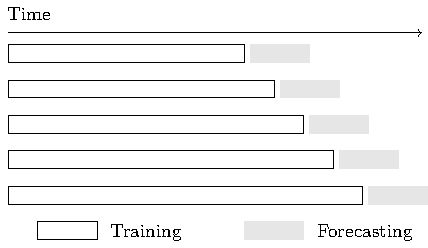
\includegraphics[width=0.8\textwidth]{../manuscript/figures/rolling_window.pdf}
\end{figure}
\end{frame}

\begin{frame}{The DFR algorithm: constructing $\hat{\boldsymbol{\pi}}$ }

    We construct the incoherent base forecasts $\hat{\boldsymbol{\pi}}$ by assuming the independence of univariate base forecasts.

    \begin{outline}[enumerate]
        \1 Generate predictive distributions for each time series in the hierarchy using arbitrary univariate forecasting model.
        \1 Construct the joint distribution by assuming independence.
    \end{outline}

    \begin{block}{Example}$\hat{\boldsymbol{\pi}}_{Y_1} = [0.4, 0.6]'\quad \hat{\boldsymbol{\pi}}_{Y_2} = [0.3, 0.7]' \quad \hat{\boldsymbol{\pi}}_{Y_3} = [0.2, 0.2, 0.6]'$

        $
          \hat{\pi}_{(001)} = Pr(Y_1=0) \times Pr(Y_2=0) \times Pr(Y_3=1) =  0.024
        $

        \[\begin{aligned}
          \hat{\boldsymbol{\pi}} = [&0.024,0.056,0.036,0.084, \\ &0.024,0.056,0.036,0.084, \\ &0.072,0.168,0.108,0.252]'
        \end{aligned}\]
    \end{block}
\end{frame}


\begin{frame}{The DFR algorithm}
\begin{figure}
    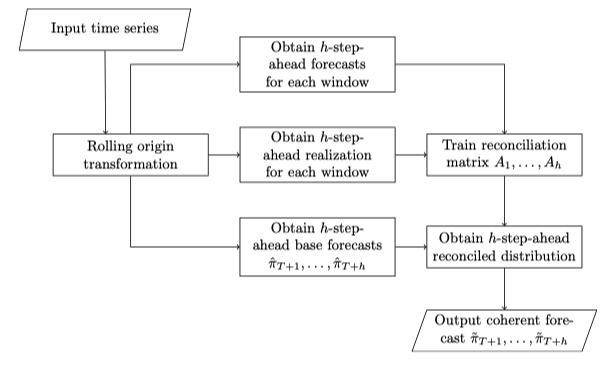
\includegraphics[width=0.9\textwidth]{figures/dfr.png}
    \caption{Flowchart of the DFR algorithm}        
\end{figure}
\end{frame}


\begin{frame}{Stepwise DFR (SDFR): handling high-dimensional hierarchy}
    \begin{outline}
    \1 The number of unknown parameters in $\mathbf{A}$ grows exponentially as the number of time series and the cardinality of domains of bottom-level series grow.
    \1 We propose the Stepwise DFR (SDFR) algorithm to deal with this problem.    
    \begin{figure}
    \centering
    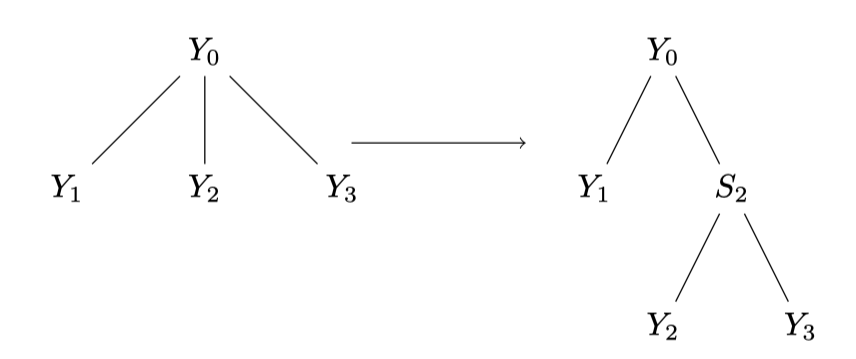
\includegraphics[width=0.6\textwidth]{figures/sdfr.png}    
    \end{figure}

    \1 It reduces the number of unknown parameters from exponential level to cubic level.
    \end{outline}
    
\end{frame}


\begin{frame}{Stepwise DFR (SDFR): handling high-dimensional hierarchy}
    \begin{figure}
        \centering
        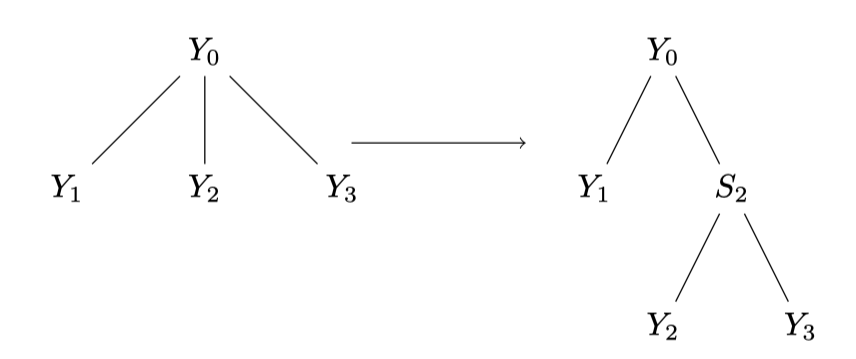
\includegraphics[width=0.8\textwidth]{figures/sdfr.png}    
    \end{figure}

\begin{enumerate}
    \item Decompose the big hierarchy into multiple small sub-hierarchies.
    \item Train the reconciliation model for each sub-hierarchy.
    \item Combine the reconciled forecasts together under assumptions.
    \[
      P(Y_0, Y_1, Y_2, Y_3) = P(Y_0, Y_1, S_2) P(Y_2, Y_3|S_2)  
    \]
\end{enumerate}
\end{frame}



\begin{frame}{Stepwise DFR (SDFR): handling high-dimensional hierarchy}
\begin{figure}
\centering
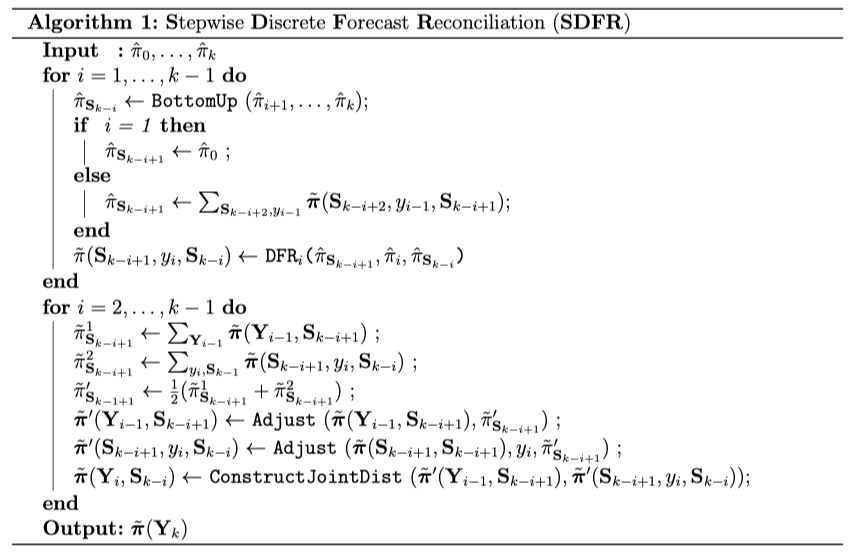
\includegraphics[width=\textwidth]{figures/alg_sdfr.png}
\end{figure}
\end{frame}





\begin{frame}{Discrete Bottom-up}
\begin{outline}
\1 The discrete bottom-up method constructs a coherent distribution by assuming independent bottom-level forecasts. 
\1 This method follows the same procedure as constructing base forecasts explained earlier except that the base forecasts of aggregated series are excluded.
\1 The mean point forecasts obtained from this coherent distribution’s marginal distribution are identical to those obtained by directly aggregating mean forecasts of bottom-level series.

\begin{block}{Example}  
\[
    \begin{aligned}
        \hat{\boldsymbol{\pi}}_{Y_1} &= [0.4, 0.6]'\quad \hat{\boldsymbol{\pi}}_{Y_2} = [0.3, 0.7]' \\
        \tilde{\pi}_{(000)} &= Pr(Y_1=0) \times Pr(Y_2=0) = 0.12      \\
        \tilde{\boldsymbol{\pi}} &= [0.12, 0.28, 0.18, 0.42]'
    \end{aligned}
\]
\end{block}
\end{outline}
\end{frame}


\begin{frame}{Discrete Top-down}

    The discrete top-down method extends the traditional top-down by proportionally disaggregating the probabilities of each point of the total series into all possible coherent points, using a ratio computed from historical occurrences.

    \begin{block}{Example}
        40 $(1, 0, 1)$ and 60 $(0, 1, 1)$ observed in the history.
        \[
            \begin{aligned}
                \hat{\boldsymbol{\pi}}_{Y_3} &= [0.2, 0.3, 0.5]' \\   
                \tilde{\pi}_{(011)} &= Pr(Y_3=1)\times\frac{60}{60+40} = 0.18\\
                \tilde{\boldsymbol{\pi}} &= [0.2, 0.18, 0.12, 0.5]'
            \end{aligned}
        \]
    \end{block}
\end{frame}

\section{Simulation}

\begin{frame}{Simulation in cross-sectional setting}
\begin{itemize}
    \item $\mathcal{D}(Y_1) = \{0, 1\}, \mathcal{D}(Y_2) = \{0, 1\}, Y_3 = Y_1 + Y_2$
    \item We produce and evaluate one-step-ahead forecast in this experiment.
    \item For each binary series, we generate $480$ observations; expanding window strategy yields $330$ samples for training and $30$ samples for testing.
    \item The performances for each time series are evaluated based on the average Brier scores of test samples.
    \item The base probabilistic forecasts are obtained using the binomial AR(1) model.
    \item The procedure was repeated $1000$ times.
\end{itemize}
\end{frame}

\begin{frame}{Simulation in cross-sectional setting}
    \begin{table}
        \centering
        \caption{Average Brier score ($\times 10^{-2}$) of $1000$ simulations for cross-sectional setting}
        \begin{tabular}{lcccc}
        \toprule
        & Base & DBU & DTD & DFR \\\midrule
        $Y_1$ & 25.4 & 25.4 & 34.9 & \textbf{24.4} \\
        $Y_2$ & 27.8 & 27.8 & 34.8 & \textbf{25.7}\\
        $Y_3$ & 49.7 & 49.5 & 49.7 & \textbf{42.0} \\
        $\mathbf{Y}$ & 74.4 & 47.8 & 56.1 & \textbf{44.0} \\
        \bottomrule
        \end{tabular}
      \end{table}
\end{frame}


\begin{frame}{Simulation in temporal setting}

\begin{figure}
\centering
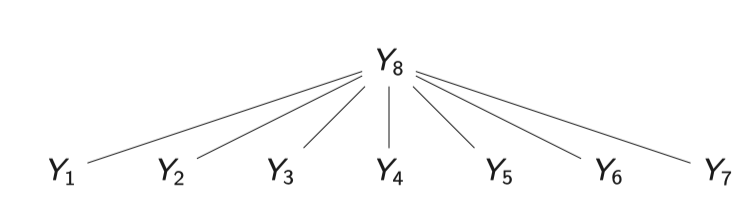
\includegraphics[width=\textwidth]{figures/temporal.png}
\end{figure}

\begin{itemize}
    \item We construct a weekly-daily temporal hierarchy in this simulation.
    \item $\mathcal{D}(Y_i) = \{ 0, 1 \} , i = 1, . . . , 7$.
    \item SDFR is used in this simulation to handle the big hierarchy.
\end{itemize}

\end{frame}


\begin{frame}{Simulation in temporal setting}
    \begin{table}
        \centering
        \caption{Average Brier score ($\times 10^{-2}$) of $1000$ samples for temporal setting.}
        \begin{tabular}{lcccc}
        \toprule
         & Base & DBU & DTD & SDFR \\\midrule
        $Y_1$ & \textbf{40.8} & \textbf{40.8} & 49.4 & 41.0 \\
        $Y_2$ & \textbf{41.4} & \textbf{41.4} & 49.6 & 41.6\\
        $Y_3$ & \textbf{42.1} & \textbf{42.1} & 49.9 & 42.1\\
        $Y_4$ & 43.0 & 43.0  & 50.0          & \textbf{42.8}\\
        $Y_5$ & 43.6 & 43.6  & 50.2          & \textbf{43.1} \\
        $Y_6$ & 44.0 & 44.0  & 50.3          & \textbf{43.3} \\
        $Y_7$ & 44.3 & 44.3  & 50.3          & \textbf{43.9} \\
        $Y_8$ & \textbf{82.6} & 83.5          & \textbf{82.6} & 83.1\\
        $\mathbf{Y}$ & 99.5 & 97.8  & 99.4          & \textbf{97.7} \\
        \bottomrule
        \end{tabular}
    \end{table}
\end{frame}

\section{Empirical study}

\begin{frame}{Forecasting crime number in Washington D.C.}
\begin{itemize}
    \item The dataset contains $231$ weekly time series of offence crime numbers from 2014 to 2022; each time series corresponds to one census tracts in Washington D.C.
    \item We construct two-level temporal hierarchies (i.e., weekly and four-weekly) and forecast the offence numbers in the next four weeks for each time series.
    
    \item Samples whose forecast origin starts from 2022 are used for evaluation.
    \item Base probabilistic forecasts are produced using integer-valued GARCH models.
    \item DFR are used to reconcile the forecasts.
\end{itemize}    
\end{frame}

\begin{frame}{Forecasting crime number in Washington D.C.}
\begin{figure}
\centering
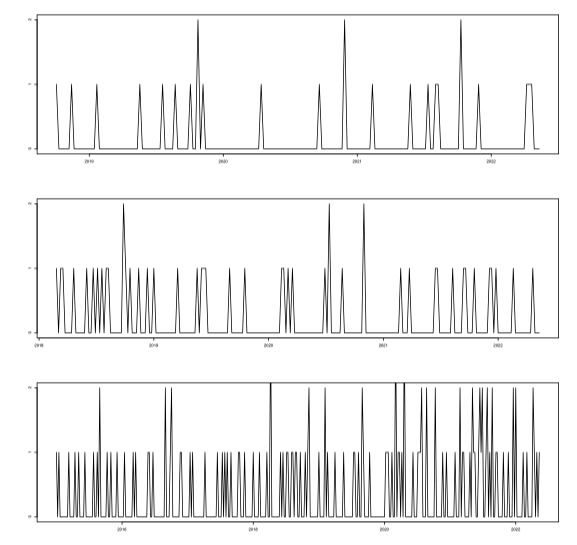
\includegraphics[width=0.65\textwidth]{figures/dc.png}
\caption{Example time series}
\end{figure}
\end{frame}


\begin{frame}{Forecasting crime number in Washington D.C.}
\begin{table}[h]
    \centering
    \caption{Summarised Brier Score($\times 10^{-2}$) of test samples in crime forecasting application.}
    \resizebox{\textwidth}{!}{
    \begin{tabular}{ccccccccc}
    \toprule
    &\multicolumn{4}{c}{Mean}
    & \multicolumn{4}{c}{Median} \\ \cmidrule(lr){2-5} \cmidrule(lr){6-9}
        & Base & DBU & DTD & DFR &  Base & DBU & DTD & DFR \\\midrule
    Total & 58.47 & \textbf{58.07} & 58.47 & 58.12 & 66.64 & 65.28 & 66.64 & \textbf{64.75} \\
    Bottom & 34.41 & 34.41 & 34.80 & \textbf{34.30} & 13.73 & 13.73 & 13.28 & \textbf{10.82}\\
    Hierarchy & 73.87 & \textbf{67.87} & 68.33 & 67.97 & 97.66 & 92.70 & 93.08 & \textbf{92.42}\\
    \bottomrule
    \end{tabular}}
    \end{table}
\end{frame}

\begin{frame}{Forecasting crime number in Washington D.C.}
\begin{figure}
\centering
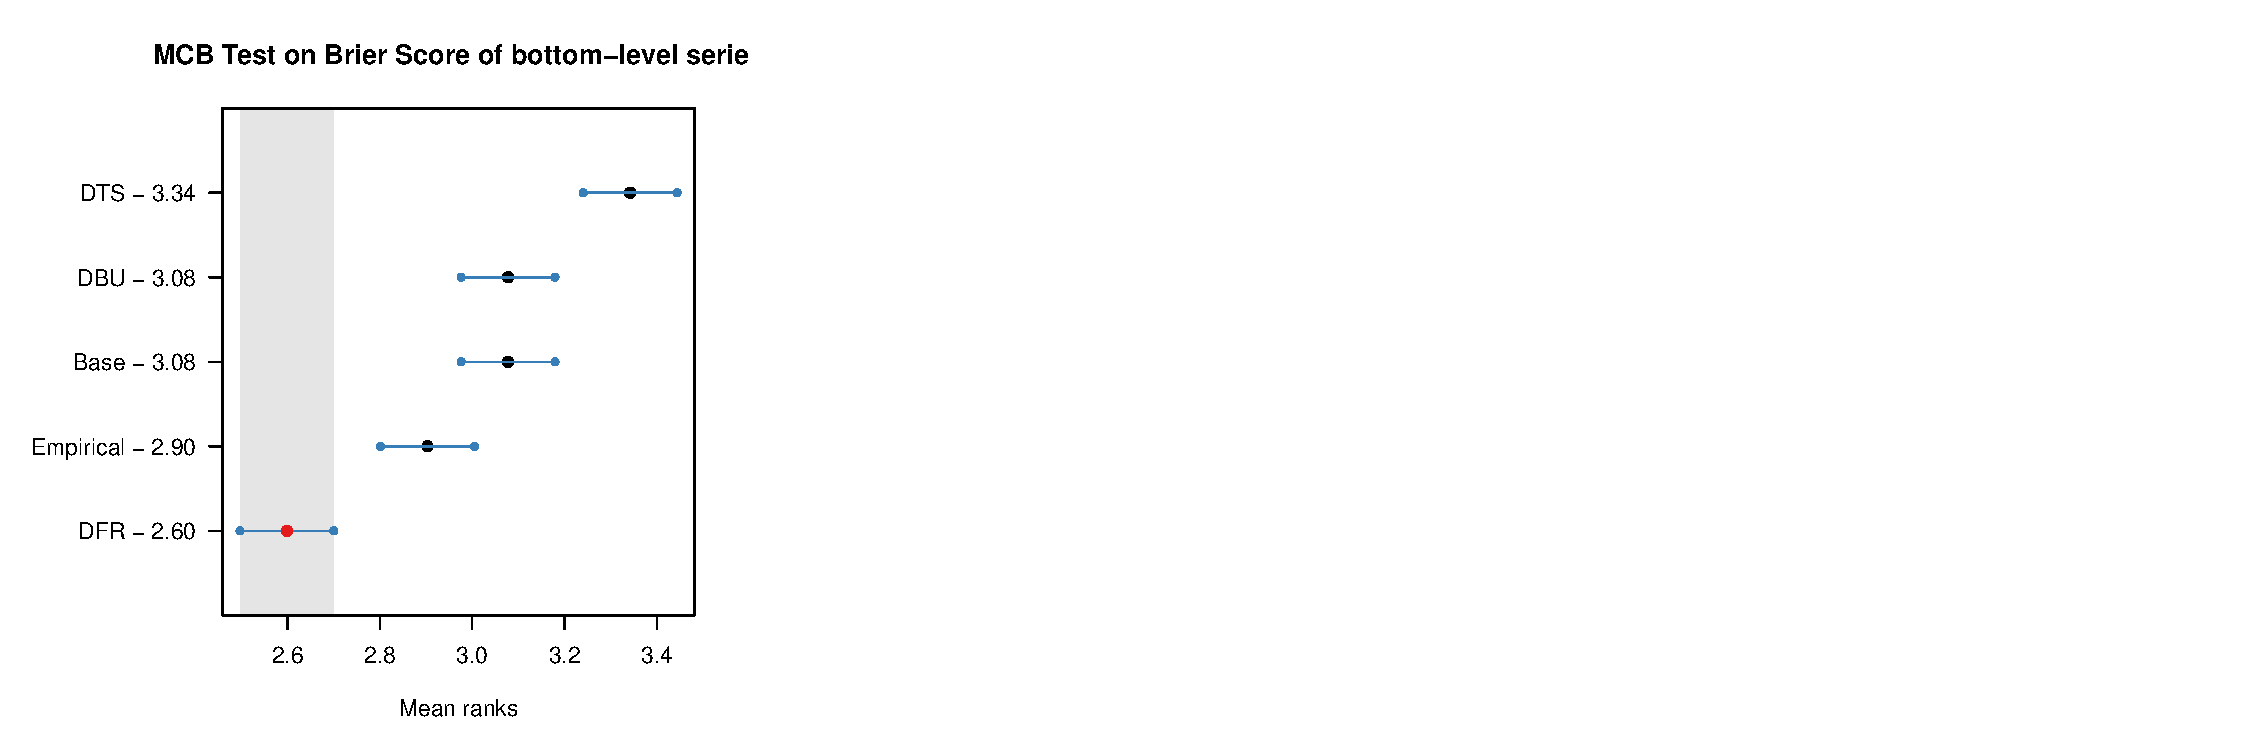
\includegraphics[width=\textwidth]{../manuscript/figures/dc_crime_mcb.pdf}
\caption{MCB test results}
\end{figure}
\end{frame}

\section{Conclusion}

\begin{frame}{Conclusion}
    \begin{itemize}
        \item We develop a novel forecast reconciliation framework for count hierarchical time series, which involves assigning probabilities from incoherent points to coherent points.
        \item We further propose a linear reconciliation algorithm that minimises Brier score of reconciled probabilistic forecasts.
        \item To address the exponential growth of the domain, we introduce a stepwise discrete reconciliation algorithm by breaking down a large hierarchy into smaller ones.
        \item Our DFR and SDFR algorithms produce coherent probabilistic forecasts and improve forecast accuracy, as shown in simulation and empirical studies.
    \end{itemize}
\end{frame}


{\setbeamertemplate{footline}{}
\begin{frame}
\begin{minipage}[t][0.8\textheight][c]{\textwidth}
\centering
\fontsize{15}{18}\selectfont
Thank you!

Any questions/suggestions/comments?    

\end{minipage}


Paper: \url{https://arxiv.org/abs/2305.18809}

Package: \url{https://github.com/AngelPone/DiscreteRecon}

\end{frame}}

\end{document}
